\section{Design of \toolname} \label{design}

This section first defines terminology and notations used throughout this
work and then details the design of the \toolname framework and its
work flow.
\vspace{-1.5mm}
\subsection{Compiler Flag Space Construction}

%how to extract interactions automatically
Modern optimizing compilers feature many internal optimization passes
and expose several hundreds of command-line flags to trigger and
parameterize them.  Each flag can be viewed as a variable with two or
more valid values, i.e., a flag could either be a binary switch
to turn on/off a certain optimization (e.g., loop unrolling and loop
tiling), or a multi-valued parametric option to set pass-specific
parameters (e.g., thresholds for function inlining and algorithmic
variants of register allocation).
%
%compiler flag vector, compiler flag space
The set of all flags composes a space called the compiler optimization
space ($COS$), in which each point is a set of instantiated flags, a
so-called compiler flag vector or compilation vector ($CV$).

Suppose there are $N$ compiler flags, denoted as $F_i$
$(1\leq{i}\leq{N})$.  Further suppose $F_i$ has $n_i$ possible values
$f_{i1}, f_{i2}, ..., f_{i{n_i}}$.  Then a sample $CV$ is represented
as $(F_1=f_{1k_{1}}, F_2=f_{2k_{2}}, ..., F_N=f_{Nk_{N}})$ or simply
$(f_{1k_{1}}, f_{2k_{2}}, ..., f_{Nk_{N}})$, where
$1 \leq{k_i} \leq{n_i}$.  Thus, there are in total
$C_0=\prod_{i=1}^{N} n_{i}$ $CVs$, each of which could be used to
compile all source files of a program in a traditional compilation
model (see \Cref{fig:cm1}).

\begin{figure}
\centering
\subfloat[]
{
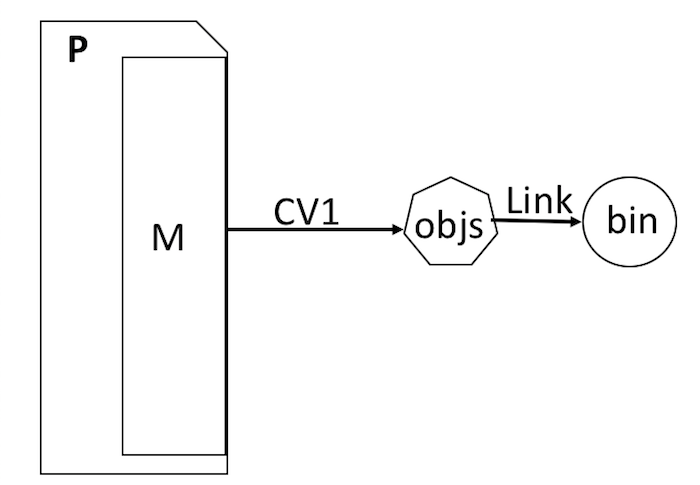
\includegraphics[scale=.2]{figures/cm1.png}
\label{fig:cm1}
}
\subfloat[]
{
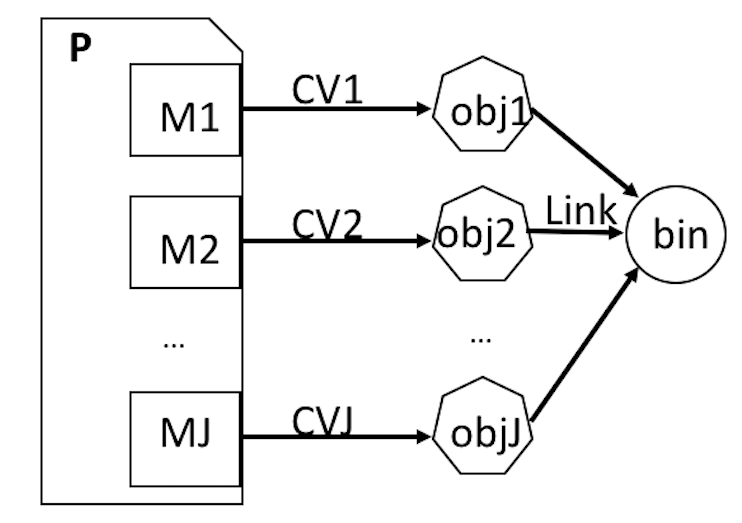
\includegraphics[scale=.2]{figures/cm2.png}
\label{fig:cm2}
}
\caption{Comparison of compilation models. a) A traditional compilation
  model with the same $CV$ to compile all modules; b) \toolname's
  compilation model with different $CVs$ to compile
  different modules.}
\label{fig:cms}
\end{figure}


\if 0
\begin{figure}
\centering
\subfloat[Part 1][]{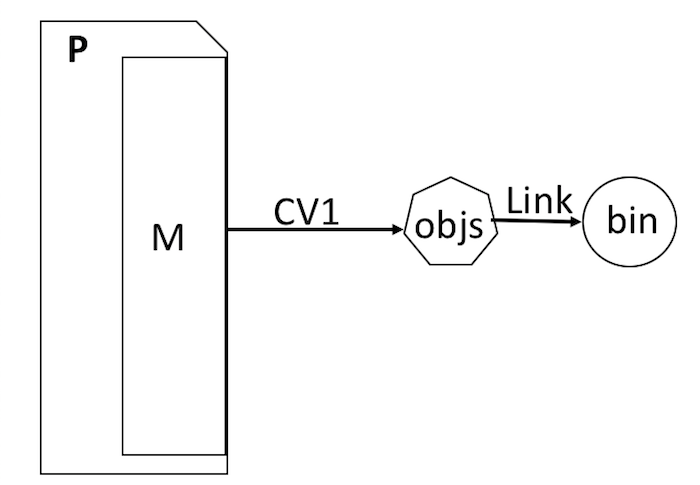
\includegraphics[width=0.4\textwidth]{figures/cm1.png}
\label{fig:cm1}}
\subfloat[Part 1][]{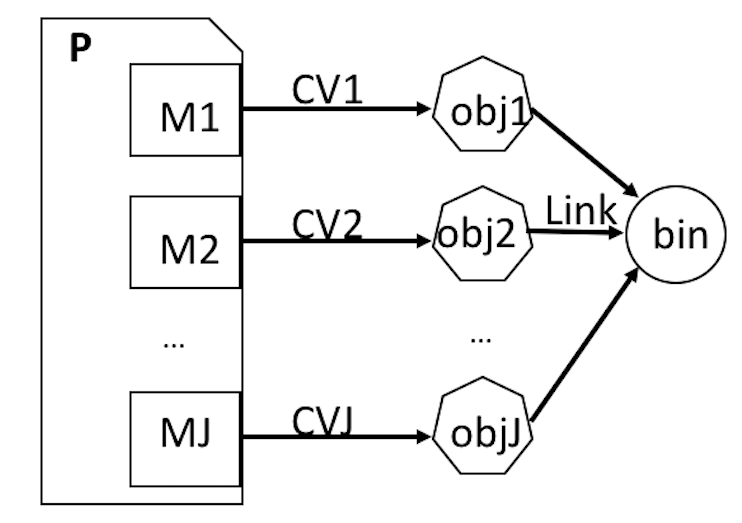
\includegraphics[width=0.4\textwidth]{figures/cm2.png}
\label{fig:cm2}}
\caption{Comparison of compilation models. a) A traditional compilation
  model with the same $CV$ to compile all modules; b) \toolname's
  compilation model with different $CVs$ to compile
  different modules.}
\label{fig:cms}
\vspace{-4mm}
\end{figure}
\fi


\begin {table}[t]
%\nocaptionrule
\caption{Symbol definitions}
\label{table:notations}
%\vspace{2pt}
\centering
\footnotesize
\begin{tabular}{ p{2cm}p{14cm} }
\hline
\textbf{Notation} &  \textbf{Definition} \\ \hline
$N$ & number of compilation flags/options\\ \hline
$F_i$ & i-th compilation options, $(1\leq{i}\leq{N})$\\ 
\hline
$n_i$  & number of possible values for $F_i$ \\ \hline
$f_{ih}$  & h-th value of $F_i$, $(1\leq{h}\leq{n_i})$ \\ 
\hline
$COS$ & Compiler optimization space; Cartesian
   product of values possible for all options:
   ($F_1=f_{11}, F_1=f_{12}, ..., F_1=f_{1n_1})~\times$
    ($F_2=f_{21}, F_1=f_{22}, ..., F_1=f_{2n_2})~\times$
   $\space(...)~\times$ ($F_N=f_{N1}, F_1=f_{N2}, ..., F_1=f_{Nn_N})$\\ \hline
$COS_{new}$& COS for our fine-grained approach\\ \hline
$CV$ & Compilation vector, an instance in $COS$, e.g.,
  $CV=(F_1=f_{11}, F_2=f_{22}, ..., F_N=f_{N3})$\\ \hline
% & \\
 $C_0$ & $\prod_{i=1}^{N} n_{i}$, number of $CV$s in $COS$ \\ \hline
%& \\
$M$ & A \textbf{compilation module} within which source file(s) are compiled with the same $CV$ \\ \hline
%& \\
 $P$  & A source program composed of one or multiple \textbf{compilation module}s\\ \hline
%  & \\
 $J$ & number of modules M in $P$; is a program-specific variable \\ \hline
% & \\
 $C_1$ & ${C_0}^J$, number of $CV$s in $COS_{new}$ \\ \hline
%  & \\
 $M_j$ & j-th compilation module of $P$, $(1\leq{j}\leq{J})$\\
%\hdashline
% $CV_j$ & CV for $M_j$, $(1\leq{j}\leq{J})$\\
%\hdashline
%CVV & vector of all CVs to compilation a program in \\
%& fine-grained compilation model \Cref{fig:cm2}, \\
%  & \\
\hline
 $K$  & number of $CV$ samples \\ \hline
%  & \\
 $P_k$  & $P$ compiled with k-th set of $CVs$  for a \\& given method \\ \hline
%  & \\
 $M_{jk}$  & j-th $M$ of $P_k$.\\ \hline
%  & \\
 $CV_{jk}$  & $CV$ for $M_{jk}$ \\
\hline
%  & \\
 $MCV_k$  & \textbf{program compilation configuration}, configuration of per-module $CV$ for $P_k$;
  If $P_k$ is composed of $(M_{1k}, M_{2k}, ..., M_{Jk}),$
  and its $MCV_k$ is $(CV_{1k}, CV_{2k}, ... ,CV_{Jk}),$ it
  means that every source file within $M_{1k}$ is
  compiled with $CV_{1k}$ and so on\\
\hline
%  & \\
$T_{jk}$  & total accumulated runtime for $M_{jk}$ \\
 \hline
%  & \\
$T_k$  & end-to-end runtime for $P_k$ and $T_k=\sum\limits_{j=1}^{J} T_{jk}$\\
\hline
%  & \\
$T_{O3}$  & end-to-end runtime for $P$ compiled with O3 \\
 \hline
\end{tabular}
\end {table}

Given a program $P$, a traditional compilation model (shown in
\Cref{fig:cm1}) treats all its source files as a single
compilation module $M$, within which the source files are
compiled with the same $CV$.
% Conceptual diagram:
In contrast, as shown in \Cref{fig:cm2}, \toolname divides program $P$
into $J$ compilation modules $M_1, M_2, ..., M_J$; these modules are
created based on the time spent in various regions, in particular
loops, of the program P.  \toolname then compiles $M_j$ with a $CV$,
which is determined independently from other modules and links all
object files to produce the executable.  Our hypothesis is that
different compilation modules may need different $CV$s to obtain the
best performance due to their diverse code structures.
%and the fact that compiler built-in cost models or heuristics do not always make the best decisions.

However, the primary challenge is that the new search space size
$COS_{new}$ increases significantly from $C_0$ to $C_1={C_0}^J$, since
each module can be compiled independently with a different $CV$ in
$COS$.  Exhaustive search is not a viable option within such an
excessively large space while predictive modeling based on machine
learning requires a significant amount of training data and meaningful
features to begin with~\cite{FursinMGL15}. To address this challenge, we design and implement
several algorithms within our framework, as detailed in the rest of this
section.  To facilitate the discussion, we define the notations
in \Cref{table:notations}. We do not differentiate between a program source code
    module and its corresponding object/binary module. Therefore,
    $P_k$ ($M_{jk}$) may represent the source code module or compiled
    program object/binary module, depending on the context.

\subsection{Space Search Algorithms}

\subsubsection{Coarse-grained Random Search}

Coarse-grained Random Search (denoted as Random) does not modify program
source code. As shown in
\Cref{fig:csr}, It utilizes random search within the traditional
compilation model (\Cref{fig:cm1}), i.e., it applies a single $CV$ to
all source files for any program $P$.  In step \textcircled{1}, 1000
$CV$ samples are randomly selected from $COS$~\cite{opentuner}.  In
step \textcircled{2}, each $CV$ is used to compile $P$ to obtain a
code variant, $P_i$.  Thus, we obtain 1000 code variants in total.  In
step \textcircled{3}, runtimes are collected for all code variants.
In the end, the code variant with the least runtime is selected as the final result.
%Coarse-grained random search does not modify $P$'s
%source code, we denote \\it as $R$.
The size of its search space is
$C_0$, as in \Cref{table:notations}.
%, and pseudo code is presented in \textbf{\Cref{alg:csr}}.
\begin{figure}
\centering
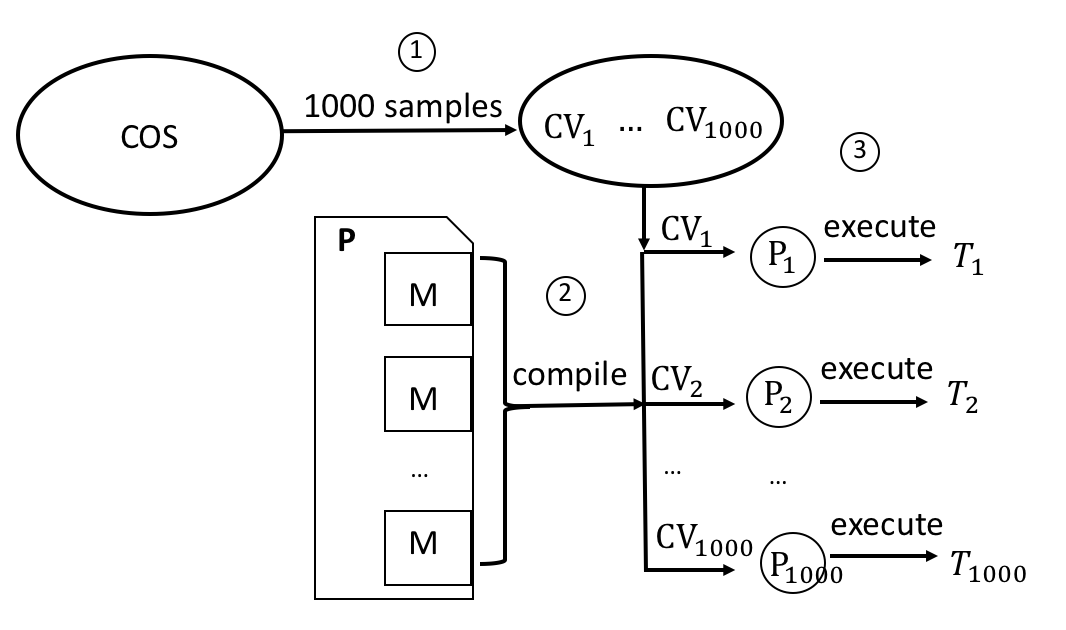
\includegraphics[width=0.6\textwidth]{figures/r_origin}
\vspace{-4mm}
\caption{Overview of Coarse-grained Random Search. $CV_k$ and $P_k$
  with minimal runtime $T_k$ is its final result.}
\label{fig:csr}
\vspace{-4mm}
\end{figure}
\subsubsection{Fine-grained Random Search}

As shown in \Cref{fig:fr}, Fine-grained Random search (denoted as
$FR$) begins with profiling an input program $P$ to identify hot loops
and outlines each of them into a separate source files so that there
are $J$ compilation modules.  After that, $J$ $CV$s are randomly
selected from 1000 pre-sampled $CV$s.  Each selected $CV$ is then used
to compile one of the $J$ modules of $P$.

\iffalse
\begin{algorithm}
\DontPrintSemicolon
\SetAlgoLined
\SetKwInOut{Input}{Input}
\SetKwInOut{Output}{Output}
\Input{$COS, K, P, T_{O3}$}
\Output{$speedup, CV$}
\BlankLine
$k = 0$, $T= [ ]$, $CV$s$ = []$ \;
$CV$s = randomSample ($COS, K$)\;
\While{ $k < K$ }{
    compile $P$ with $CVs[k]$ to generate $P_k$\;
    run $P$ to measure $T_k$ \;
    $T[k] = T_k$ \;
    $k$++
}
$k = \operatorname*{argmin}_k {\{T[k]}$ ${ | 1\leq{k}\leq{K}\}}$ \;
\;
$CV$ = $CVs[k]$\;
speedup = $T_{O3}/T[k]$ \;
\caption{Coarse-grained Random Search}
\label{alg:csr}
\end{algorithm}
\fi

Note that the selection of $J$ CVs and compilation is performed 1000
times in step \textcircled{3} to generated 1000 code variants $P_1$,
..., $P_{1000}$, which are executed to collect runtimes $T_1$, ...,
$T_{1000}$.  In the end, $FR$ reports the code variant with the
minimum runtime as the best version.  
The detailed algorithm is
presented in \Cref{alg:fr}.

\begin{figure}
\centering
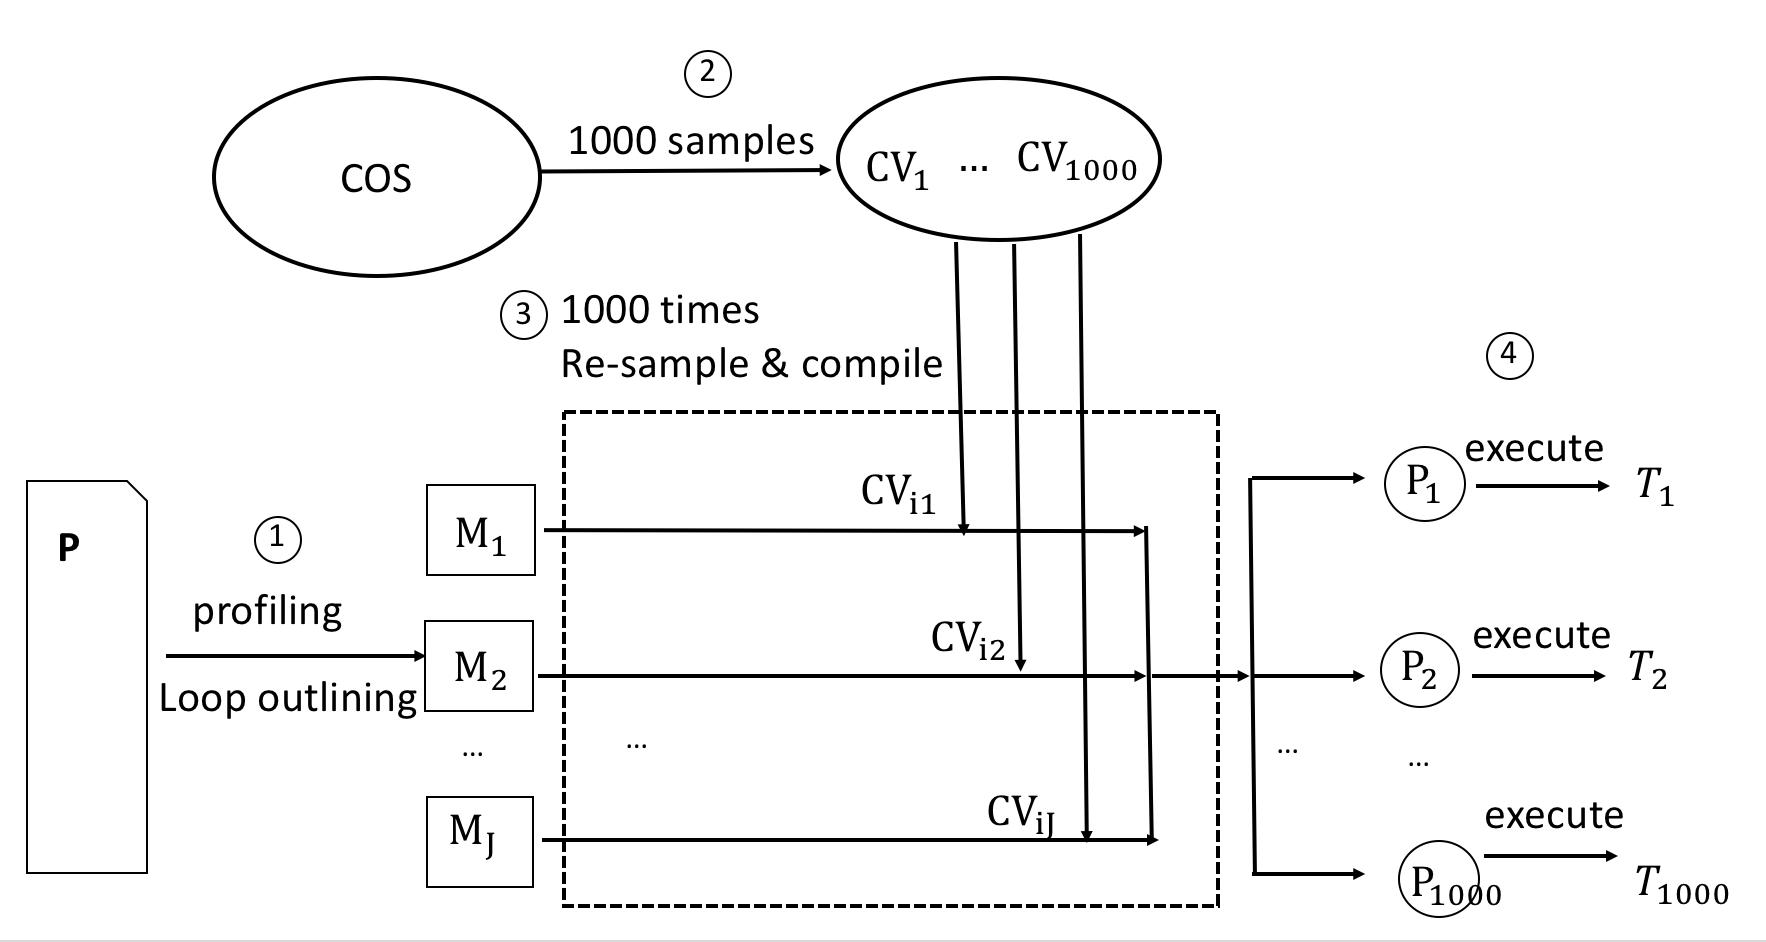
\includegraphics[width=0.6\textwidth]{figures/fr}
\caption{Fine-grained Random Search. Step \textcircled{3} (re-sample \& compile) is performed 1000 times.}
\label{fig:fr}
\end{figure}

\begin{algorithm}
\DontPrintSemicolon
\SetAlgoLined
\SetKwInOut{Input}{Input}
\SetKwInOut{Output}{Output}
//For FR, $CV_{pruned}$ initially is empty\;
\Input{$COS, K, P, T_{O3}$}
\Output{$speedup, CV$}
\BlankLine
$T= [ ]$, $tempCVs=[][]$, $CV$s$ = []$ \;
%\uIf{$CV_{pruned}$ is []}{
//returns K random samples from $COS$\;
$CV$s = randomSample ($COS, K$)\;
%}\Else{
%$CVs = CV_{pruned}$\;
%CFR=true
%}
\For {$k=0$; $k < K$; $k$++}{
    tempCVs[k][] = randomSample($CV$s, $J$)\;
    \For {$j=0$; $j < J$; $j$++}{
    	compile $M_j$ with tempCVs[k][j]
    }
    link $M_1$, ..., $M_J$ to generate $P_k$\;
    run $P_k$ to measure $T_k$ \;
    $T[k] = T_k$ \;
}
$k = \operatorname*{argmin}_k {\{T[k]}$ ${ | 1\leq{k}\leq{K}\}}$ \;
$CV$ = $tempCVs[k]$\;
speedup = $T_{O3}/T[k]$ \;
\caption{Fine-grained Random Search (FR)}
\label{alg:fr}

\end{algorithm}

\subsubsection{Greedy Combination}
% Intuition of Greedy combination

$FR$ does not use the per-loop (i.e. per-module) runtime information.
However, when per-loop runtime information is available, one can
choose better $CV$s for each compilation module.  To this end, we
introduce \toolname, our per-loop runtime collection framework, shown
in \Cref{fig:framework}.  Similar to $FR$, an input program $P$ is first
divided into $J$ compilation modules.  In step \textcircled{2},
\toolname instruments modules via a light-weight~\cite{caliper} API to
measure per-loop runtime.  Then, in step \textcircled{4}, pre-sampled
$CV_1$, ..., $CV_{1000}$ are used to compile $P$ such that all modules
within $P$ are compiled with the same k-th $CV$ to generate $P_k$.  In
step \textcircled{5}, the generated 1000 code variants are then
executed to collect per-loop runtimes, which are represented as
$T_{jk}$ for accumulative runtimes per compilation module $M_j$ of
code variant $P_k$.

The intuition of Greedy Combination (denoted as $G$) is to assemble
the final executable by picking the fastest code variant for each module
and linking them together, assuming that their composition produces
the fastest executable with the shortest end-to-end runtime.  Formally,
$G$ chooses the i-th $CV$ to compile $M_j$ such that
$i = \operatorname*{argmin}_k {\{T_{jk} | 1\leq{k}\leq{1000}\}}$, and
then links all object modules to produce the target executable.  The
pseudo code for both the \toolname data collection framework and
Greedy Combination is presented in \Cref{alg:greedy}.

\begin{figure}
\centering
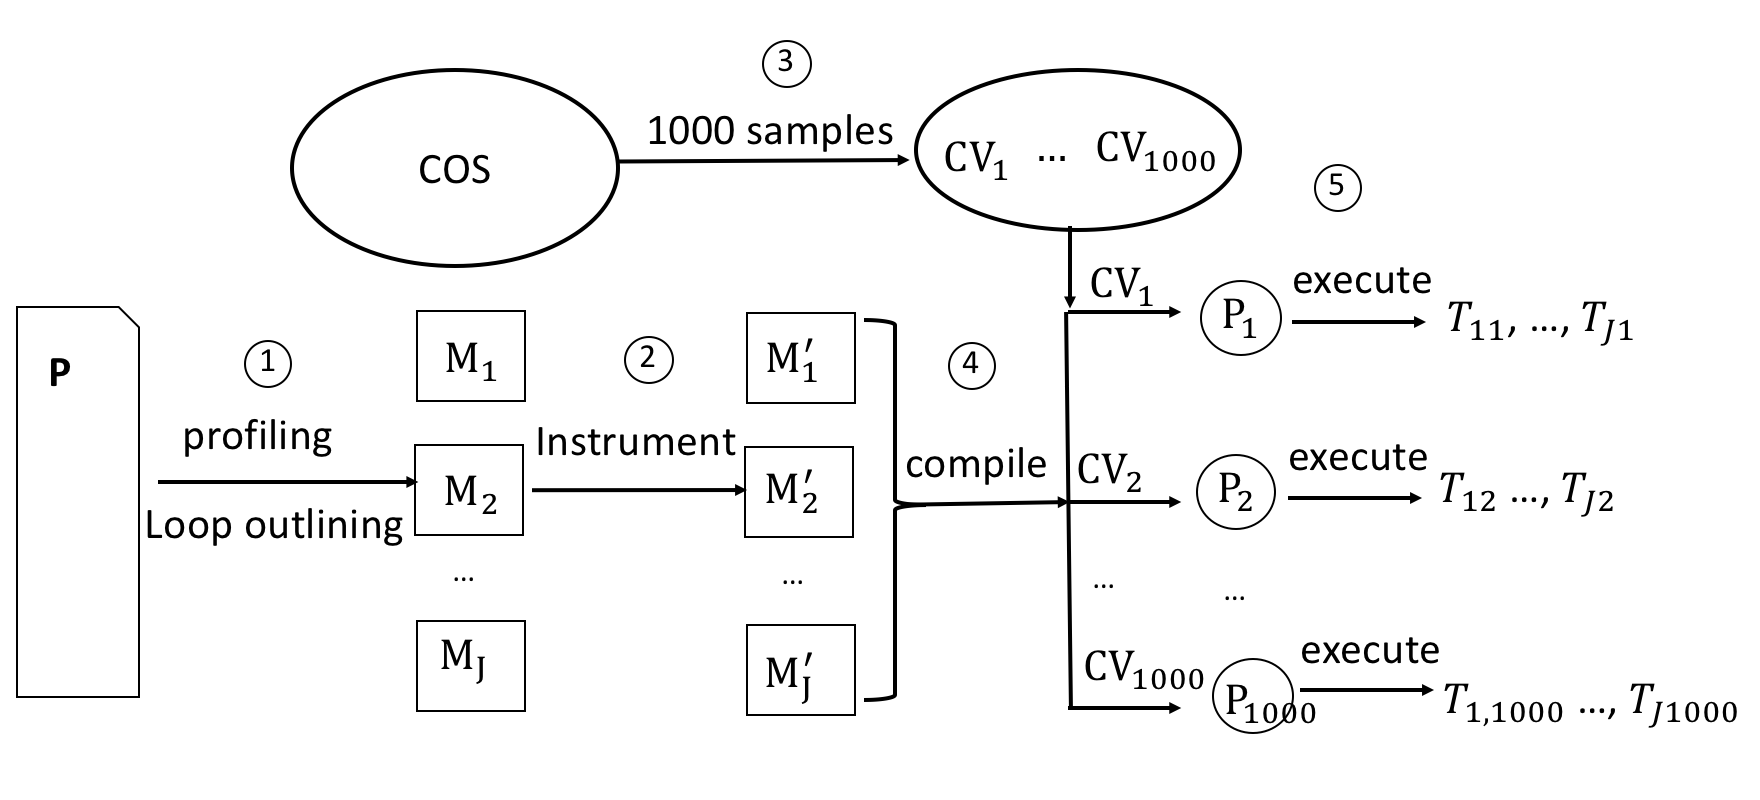
\includegraphics[width=0.6\textwidth]{figures/framework}
\caption{FuncyTuner Per-loop Runtime Data Collection Framework used for
  both Greedy Combination (\Cref{alg:greedy}) and CFR (\Cref{alg:cfr}).}
\label{fig:framework}
\end{figure}

\begin{algorithm}
\DontPrintSemicolon
\SetAlgoLined
\SetKwInOut{Input}{Input}
\SetKwInOut{Output}{Output}
\Input{$COS, K, P, T_{O3}$}
\Output{$speedup, CV$}
\BlankLine
$T = [][]$, $CV$s$ = []$, $CV_{greedy} = []$ \;
$CV$s = randomSample ($COS, K$)\;
$//$ \toolname per-loop runtime data collection\;
%\While{ $k < K$ }{
\For {$k=0$; $k < K$; $k$++}{
    compile $P$ with $CVs[k]$ to generate $P_k$\;
    run $P$ to measure $T_{1k}, ..., T_{Jk}$ \;
    \For {$j=0$; $j < J$; $j++$}{
    	$T[j][k] = T_{{j+1}k}$ \;
    }
}
//Greedy combination\;
\For {$j=0$; $j < J$; $j++$}{
	$CV_{greedy}[j] = \operatorname*{argmin}_k {\{T_{jk} | 1\leq{k}\leq{K}\}}$\;
    compile $M_j$ with $CV_{greedy}[j]$ for bject file $O_j$
}
link $O_j$s to generate target program $P_t$\;
execute $P_t$ to obtain $T_t$\;
$CV$ = $CV_{greedy}$\;
speedup = $T_{O3}/T_t$ \;
\caption{Greedy Combination (G)}
\label{alg:greedy}
\end{algorithm}

\subsubsection{Caliper-guided Random Search}

% \todo{this is unclear; algorithm seems incomplete with an if (true);
% also, i dont think algorithm 1 preserves module to module matching
% of flags}{Nice Catch!}
Similar to $G$, Caliper-guided Random Search (denoted as $CFR$)
depends on \toolname's per-loop runtime data collection to make
informed selection of $CV$s (see \Cref{fig:framework}).  However, the
key difference is that $CFR$ examines more code variants than $G$,
which only greedily assembles and evaluates 1 code variant.  Compared
to $FR$, which does not use any per-loop information and uniformly
performs a random search within the pre-sampled 1000 $CVs$ for each
hot loop, $CFR$ takes advantage of per-loop timing information and
prunes the pre-sampled search space for each hot loop before
re-sampling per-loop $CV$s (line 8 of \Cref{alg:cfr}).  The
intuition is that more performant $CV$s, which generate faster
per-loop code variants, should be kept in the re-sampled search space,
because they may have a higher chance to compose a performant target
executable.  Within this algorithmic framework, $G$ can be
considered as only selecting the top-1 $CV$s, and that $FR$ selects
all 1000 or the top-1000 $CV$s, while $CFR$ selects the top-X
($1<X<<1000$) $CV$s, all on a per-loop basis.  The pseudo code of CFR
is presented in \Cref{alg:cfr}, which also uses the \toolname per-loop
runtime data collection of \Cref{alg:greedy}.

To summarize, Random and G are the state-of-the-art search-based
algorithms while we propose FR and CFR.

\begin{algorithm}[t]
\DontPrintSemicolon
\SetAlgoLined
\SetKwInOut{Input}{Input}
\SetKwInOut{Output}{Output}
\Input{$COS, K, P, X, T_{O3}$}
\Output{$speedup, CV$}
\BlankLine
$k = 1$, $T= [ ]$, $CV$s$ = []$ , $CV_{pruned} = [][]$\;
$CV$s = randomSample ($COS, K$)\;
//step-1: \toolname per-loop data collection (Alg.\ref{alg:greedy})\;
\vspace{.5em}
//prune pre-sampled 1000 CVs\;
\For {$j=0$; $j < J$; $j$++}{
$CV_{pruned}[j][] = $ $\{{CVs[i]\,\,|\,\,T[j][i]}\,\, is\,\,among\,top\, X$-$\,smallest\,\,in\,\,T[j][0]\,,...,\,T[j][K-1]\}$
}
%\If{true}{done}
\For {$k=0$; $k < K$; $k$++}{
	//re-sampling per-loop cv in pruned space.\;
	\For {$j=0$; $j < J$; $j$++}{
    	tempCVs[k][j] = randomSample($CV_{pruned}[j]$, 1)\;
    }
    \For {$j=0$; $j < J$; $j$++}{
    	compile $M_j$ with tempCVs[k][j]
    }
    link $M_1$, ..., $M_J$ to generate $P_k$\;
    run $P_k$ to measure $T_k$ \;
    $T[k] = T_k$ \;
}
$k = \operatorname*{argmin}_k {\{T[k]}$ ${ | 1\leq{k}\leq{K}\}}$ \;
$CV$ = $tempCVs[k]$\;
speedup = $T_{O3}/T[k]$ \;
%Invoke \textbf{\Cref{alg:fr}} with (COS=[], K, P, $T_{O3}$, $CV_{pruned}$)
\caption{Caliper-guided Random Search (CFR)}
\label{alg:cfr}

\end{algorithm}
